\begin{figure}[H]
  \centering
  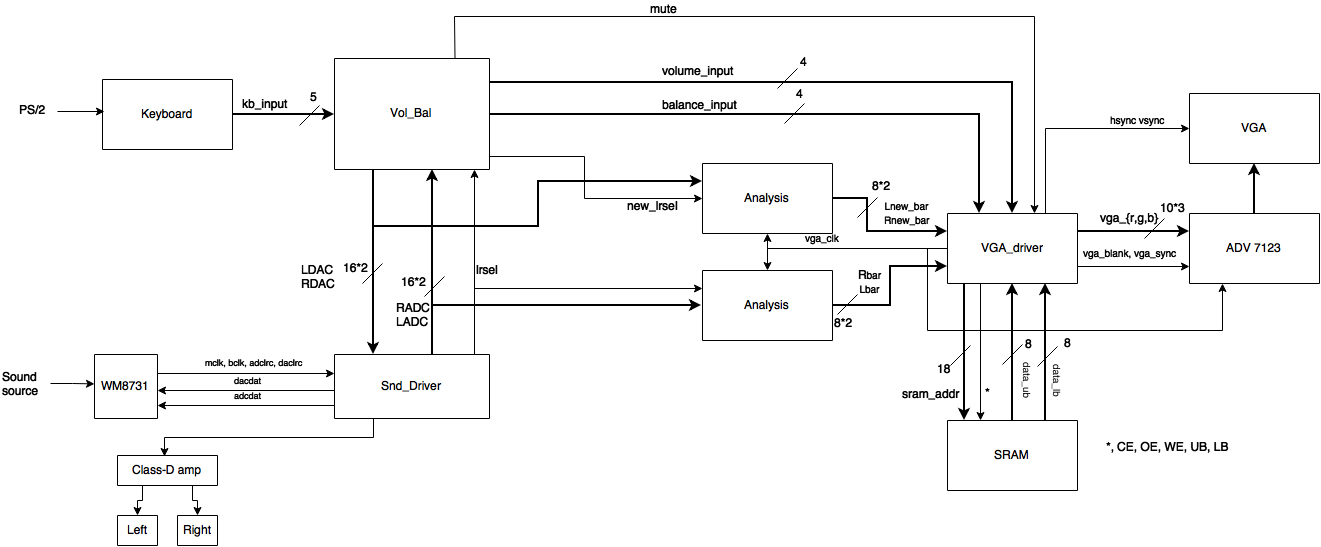
\includegraphics[width=16cm]{overview}
  \caption{G41 Project System Overview}
  \label{fig:overview}
\end{figure}

The project consists of five major modules -- \texttt{Keyboard, Vol\_Bal, Snd\_Driver, Analysis, }and \texttt{VGA\_Driver}. Presented here is an overview of the modules, and more detailed functionality is described in the \citeD.

The system takes, with help of \texttt{Snd\_Driver}, digitally encoded sound from the WM8731 chip. The sound data is passed on to the first instance of \texttt{Analysis} which provides (in order to smoothen the bar movements) low-pass filtered control signals to \texttt{VGA\_Driver:bartender} to assist the rendering of the pre-processing bar graphs done by \texttt{VGA\_Driver} as a whole. The audio data from \texttt{Snd\_Driver} is also passed on to \texttt{Vol\_Bal} which in combination with the control signals from \texttt{Keyboard} adjusts the audio balance %% mjaaa, omformuleras nog
and volume and sends it back to \texttt{Snd\_Driver} which sends signals for the class-D amplifier through the GPIO:s. The adjusted audio is also forked off to a second \texttt{Analysis} instance, which assists the post-processing bar graph rendering.

Whereas \texttt{Keyboard} and \texttt{Analysis} already are fairly small and monolithic modules, and \texttt{Snd\_Driver} and \texttt{Vol\_Bal} consists of three submodules each, \texttt{VGA\_Driver} consists of no less than twelve submodules.

\texttt{Keyboard} handles the PS/2 keyboard user input. The module filters break scan codes (F0$_{16}$, XX$_{16}$) bytewise (11 bit/byte) and compares the XX$_{16}$ byte (iff directly preceeded by F0$_{16}$) to the control key values. This approach will allow the system to respond to the regular keys (ARROW keys and END) as well as corresponding numeric keypad keys as initial E0$_{16}$ bytes are discarded. Upon a registered valid key release, a 5-bit control signal (\verb=kb_input=)is sent for a single clock cycle to \texttt{Vol\_Bal}.

\texttt{Analysis} reads the \verb=ADC= signals and lowpass filters these with a saturation time of approximately 100 ms (4096 clock cycles). These signals are converted to a graph height (in pixels) and passed on to \verb=bar_tender=.

\texttt{Snd\_Driver} have the three submodules \verb=Snd_Driver:{Ctrl,Channel_Mod}= if we count the two instances of \texttt{Channel\_Mod}. These are verbatim copies of \emph{Laboration 4}. The only difference is that the outputs are sent to GPIO pins (and from there via an i2c adapter to the class-D amp) as well as back to the WM8731 codec.

\texttt{Vol\_Bal} consists of the three submodules \verb=Vol_Bal:{Current_Vol_Bal,{Volume,Balance}_Adjustment}=. \verb=Current_Vol_Bal= reads \verb=kb_input= and updates registers representing system levels of volume, balance and mute.
\verb=Volume_Adjustment= adjusts volume according to the volume\_level input from \verb=Current_Vol_Bal=, decreasing amplitude by up to -30 dB in 3 dB decrements, and \verb=Balance_Adjustment= adjusts the audio according to system balance level, resulting in a linear scaling the incoming amplitude. The stronger a channel bias, the higher the signal reduction of the opposing channel. The affected channel loses 1/8 of the amplitude per level of bias.

\texttt{VGA\_Driver} with its submodules handles the rendering of the UI. The module is, in essence, a modified version of the module used in \emph{Laboration 3}. The most significant difference is found in the two new modules \verb=VGA_Driver:Bar_Tender= and \verb=VGA_Driver:Bar_Mixer=. \verb=Bar_Tender= uses the output from \verb=Vol_Bal= and each of the \verb=Analysis= modules along with \verb={h,v}cnt= to calculate which pixel is to be rendered and if it should be rendered from the background image or if to draw it black. The result of the calculations is the control signal \verb=render_bar=. This signal is then passed to \verb=Bar_Mixer=, which is basically a multiplexer, either forwarding the loaded background colors or a blacked out pixel depending on \verb=render_bar= from \verb=Bar_Tender=.
